% TODO Show circuit

\FloatBarrier

\begin{figure}[h!]
	\centering
	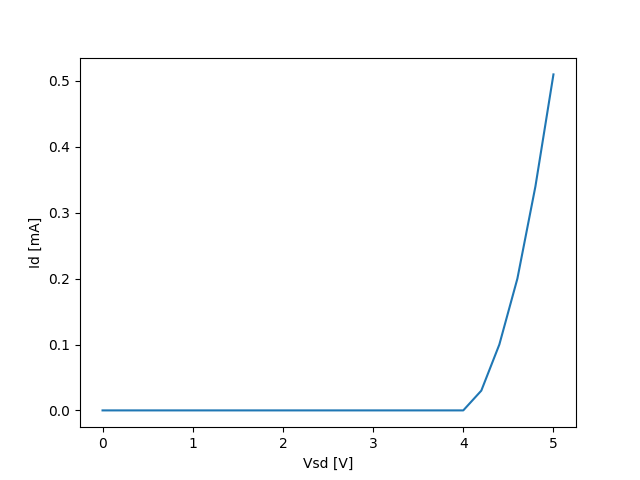
\includegraphics[scale=0.75]{../images/data_4.PNG}
	\caption{$i_{D}$ versus $V_{SD}$ for PMOS with $V_{GS} = 2.5$\si{\volt}}
	\label{fig:data_4}
\end{figure}

\FloatBarrier

One would hope to acquire similar results in figure (\ref{fig:data_4}) for the PMOS as are obtained for the NMOS.
However, the results are drastically different.
Reliable data for the $V_{GS} = 5$\si{\volt} case could not be acquired.
The CD4007 chips could likely have been damaged due to short circuits or other practical considerations, leading to the bizarre characteristics that make it act as a diode with a very high forward voltage.
